% !TEX root = ../../技术文档.tex
\section{系统整体介绍}

\subsection{系统架构}

系统由TriHaRiscv SoC与视频子系统组成，整体架构如图\ref{fig:system-architecture}所示。
SoC以支持单/双发射配置的六级RISC-V CPU为控制核心，集成NPU、片上存储和访问互连；视频子系统在FPGA顶层与SoC并列连接，完成图像采集、输入预处理和同帧全屏显示。
CPU执行裸机程序，向NPU提交绑定输入帧和工作区的整帧任务，处理检测输出并提交显示参数；NPU读取模型程序，依次执行YuNet的卷积及辅助运算。

\begin{figure}[!htbp]
\centering
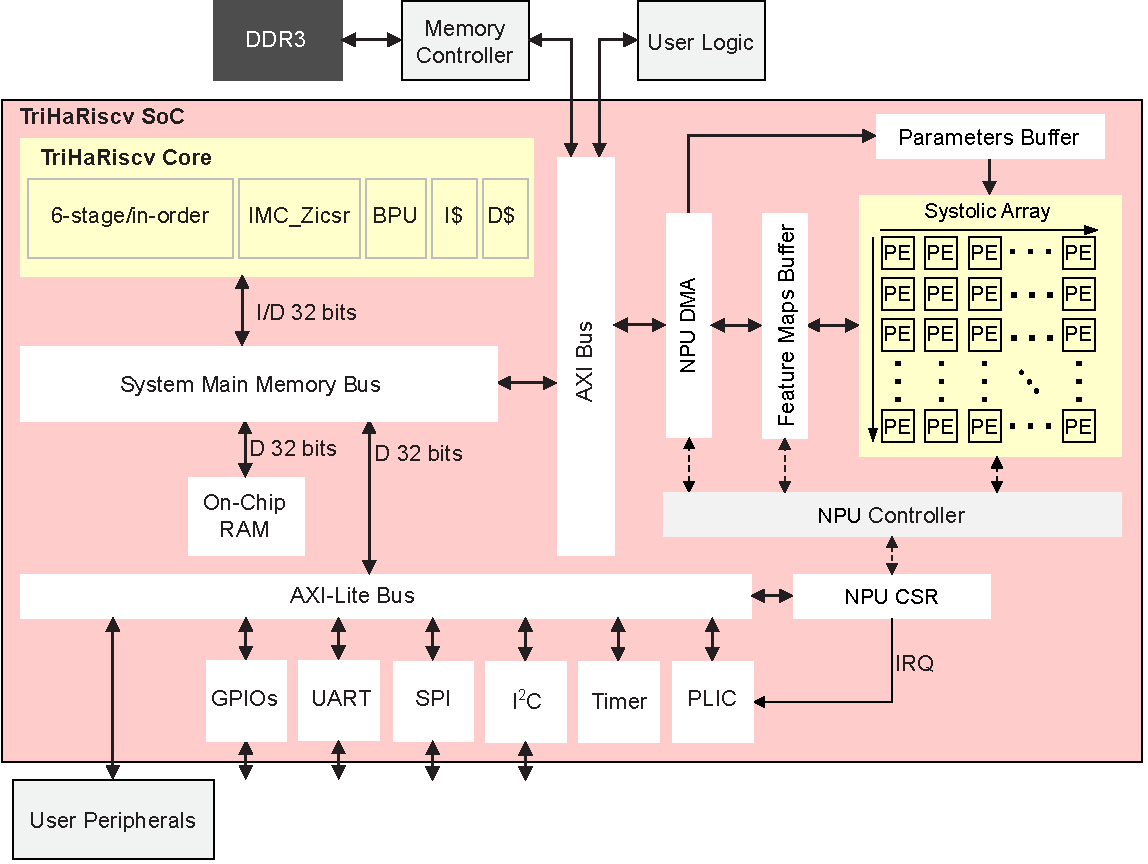
\includegraphics[width=\linewidth]{../figure/rv32-soc-page1.pdf}
\caption{TriHaRiscv异构SoC系统架构图}\label{fig:system-architecture}
\end{figure}

控制通路采用32\,bit AXI4-Lite，连接SoC内部的NPU任务与状态寄存器，并通过外部控制接口访问Video CSR。
视频DMA作为独立AXI主设备接入数据互连，与CPU访存桥和NPU DMA共享DDR访问通路，逻辑数据接口宽度为128\,bit。
Video与NPU的事件中断汇入CPU外部中断输入，应用通过寄存器轮询管理任务。Boot ROM和片上SRAM支持CPU启动，DDR按访问属性划分为CPU私有区和共享区。
DDR控制器、视频子系统及HDMI接收、发送封装均位于SoC之外，由FPGA顶层完成连接。

输入的800$\times$600 RGB888画面生成原图和320$\times$320 UINT8 BGR NCHW检测输入。
CPU对每个选定的输入帧提交一次网络推理任务，NPU依次执行各层算子并输出九个检测头，CPU完成定点解码、NMS和主人脸选择。
视频DMA将两条采集支路的数据写入DDR，显示端预取原图，经行缓存、检测框或头像合成与时序生成模块输出一路800$\times$600全屏HDMI画面。
帧控制模块在显示边界整体更新原图地址、检测框及头像参数，保持图像与检测结果的帧号一致；无人脸时输出对应原图。

\subsection{模块功能}

系统按CPU、NPU、总线、存储、外设和视频六类模块组织，视频模块在FPGA顶层与SoC连接，SoC内部模块组成如图\ref{fig:soc-modules}所示。
硬件模块通过总线和事件接口连接，裸机软件负责整帧任务调度、帧所有权管理及异常记录。

\begin{figure}[!htbp]
\centering
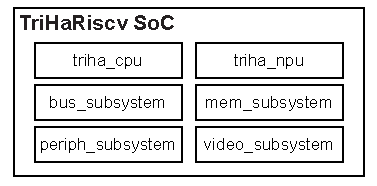
\includegraphics[width=0.5\linewidth]{../figure/rv32-soc-page2.pdf}
\caption{TriHaRiscv SoC模块图}\label{fig:soc-modules}
\end{figure}

CPU经总线模块读取模型输出、配置计算任务并提交显示记录。NPU通过DMA访问权重、输入张量和中间张量；
Video通过独立DMA写入采集数据、读取原图和头像素材。存储模块组织ROM、SRAM和DDR访问，板级控制逻辑完成模型与素材装载、接口初始化和运行状态指示。
各模块的主要功能与接口见表\ref{tbl:module-roles}。

\begin{reporttable}
\begin{longtable}{@{}p{0.25\linewidth}p{0.41\linewidth}p{0.29\linewidth}@{}}
\caption{SoC模块功能表}\label{tbl:module-roles}\\
\toprule
模块 & 主要功能 & 主要接口 \\
\midrule
\endfirsthead
\caption[]{SoC模块功能表（续）}\\
\toprule
模块 & 主要功能 & 主要接口 \\
\midrule
\endhead
\bottomrule
\endfoot
\texttt{triha\_cpu} & 执行程序、处理异常中断，运行任务调度、检测后处理和帧管理软件 & 64\,bit取指返回、32\,bit数据接口、中断输入 \\
\texttt{triha\_npu} & 读取模型图并执行普通/深度卷积及辅助算子，管理分块、缓冲与DMA & AXI4数据、AXI4-Lite整帧任务接口、完成/错误中断 \\
\texttt{bus\_subsystem} & 地址译码、访问仲裁、CPU接口桥接和错误响应 & CPU访存、AXI4及AXI4-Lite接口 \\
\texttt{mem\_subsystem} & 组织ROM、SRAM、DDR窗口及访问属性 & 片上存储接口、DDR访问接口 \\
板级控制逻辑 & 完成模型与头像串口装载、HDMI初始化及按键处理 & UART、I\textsuperscript{2}C、复位与LED \\
\texttt{video\_subsystem} & 完成全帧采集、预处理、输入格式化、全屏显示、检测框及头像合成 & 像素流、AXI4 DMA、控制寄存器、帧事件 \\
\end{longtable}
\end{reporttable}

